
\section{The \app Framework Overview}

\begin{figure*}[tbp] \centering
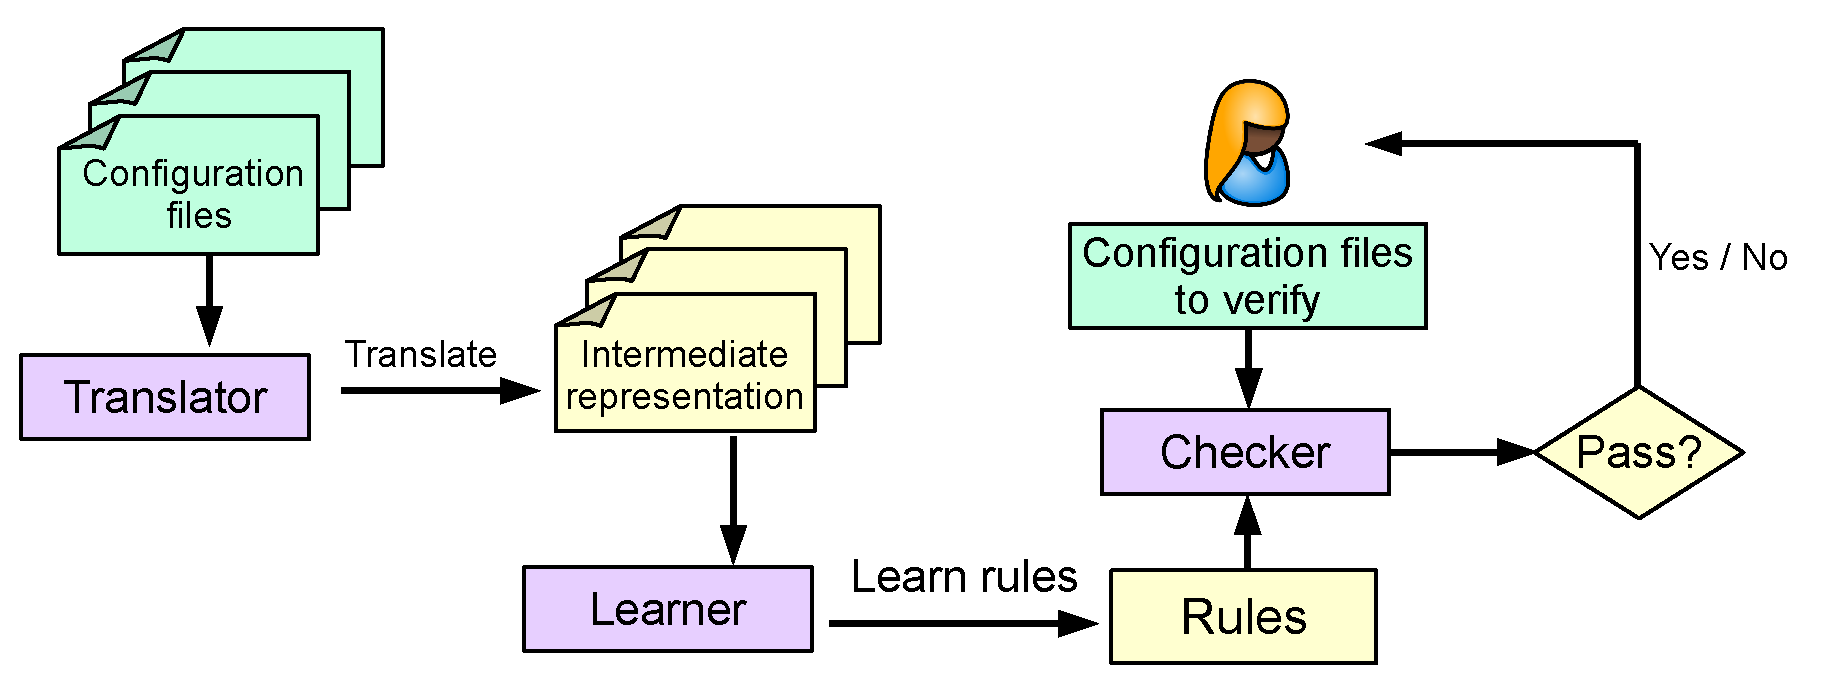
\includegraphics[width=0.68\textwidth]{figs/overview}
\caption{\app's workflow. The green boxes represent configuration files,
  including both correct general configuration files and users' input
  configuration files. The purple boxes are the components within \app.
  The yellow boxes are results generated by \app's components.}
\label{fig-overview}
\end{figure*}

Figure~\ref{fig-overview} describes an overview of our system. We start
with the assumption that we are given a number of correct configuration
files belonging to the same category, such as MySQL or Apache. 
Such files follow similar patterns, which we exploit
in a learning algorithm to build rules that
describe a language model for the files. Since the
``language'' of configuration types is untyped and unstructured, we
first parse the files and translate them into a more structured,
intermediary representation.
When running type inference on a configuration file, 
the type of a variable cannot always be fully determined from 
a single value.
We address this problem 
by introducing so called {\emph{probabilistic types}}.
Rather than giving a variable a single type, we assign several types with their probability distributions. 
We can then use these more structured files
as a training set to learn the rules. The learning algorithm
is template-based to be easily extensible. We provide an initial set of templates and the
learner learns some concrete instances from the training set. These
rules are used for detecting errors violating the learned constraints
in the files given by the user.

As an 
illustration of a simple rule that we can learn, consider a template
 $X_1 \le X_2$, where $X_1$ and $X_2$ are
integer variables. The learner might derive the rule stating that
$\texttt{mysql.max\_persistent} \le \texttt{max\_connections}$. There is a classification and taxonomy of configuration errors in the 
existing work on automated configuration troubleshooting~\cite{yin11anempirical, configdataset}. We provide templates for every class that \app can handle: we consider integer constraints, ordering
constraints, typing constraints, and constraints about correlated entries (such as ``if $X$ is present, $Y$ has to appear as well''). 
Unfortunately, we cannot handle the class of errors that rely on the analysis of the whole operating system.
Our language-based approach can only learn on sets of text files, not the system environment.



\com{
A rule R is added to the set of all rules,
  if $\exists$ learning file f s.t. R(f) is non vacuously true
That rule R is then removed from the set of all rules,
  if $\exists$ learning file f st R(f) is false.

This is accomplished in two passes.
First we collect all possible rules for every file.
Then we merge the all the rules to create our final set.
This conviently gives rise to an embarresingly parallel situation, which Haskell allows us to easily take advantage of by
  using the parallel mapping library parmap.

\begin{lstlisting}
  potentialRules = parmap findAllRules learningSet.
  finalRules = foldl1 mergeRules potenialRules
\begin{lstlisting}


Each rule is of the Attribute typeclass, which means a rule must support the following operations:
\begin{lstlisting}
class Attribute r where
  learn :: ConfigFile Common -> [r]
  merge :: [r] -> [r] -> [r] 
  check :: [r] -> ConfigFile Common -> Error
\end{lstlisting} 

}

